\documentclass[12pt, openany, twocolumn]{article}
\usepackage[utf8]{inputenc}
\usepackage[top = 1.5cm, left = 1.5cm, right =1.5cm, bottom = 1.5cm]{geometry}
\usepackage{graphicx}
\usepackage[pdfborder ={0 0 0}]{hyperref}
\usepackage{float} 

\title{In which way the use of virtual reality increases the efficiency of a learning process ?}
\author{ Aurélia Besse, Etienne Duverney, Jean-Guillaume Ponsard, Romain Junca }
\date{April 2019}

\begin{document}

\maketitle
\section{Abstract}

In this experiment, we try to see how much more effective virtual-reality-based exercises are rather than physical exercises. 
To do this, we had people play the Simon game, in both physical and virtual reality, to compare the evolution of their results. 
The results show that players have generally reached a much higher level in virtual reality than in the physical game.
On the short term, we notice the VR training show better results than the physical version of the game for memory performances. 
On the long term, we notice a great improvement with the use of the virtual reality technology. It is also possible with the physical version of the game, but most of the time, going from VR to the physical version brings a regression of the performances, whereas going from the physical version to VR brings an improvement.
Most of the test subjects also claimed that the VR version is funnier and easier than the physical version of the game.
For both short term and long term, we studied the speed of execution but we were not able to demonstrate any improvement due to too many bias.
Regarding the techonology, we were able to highlight the fact that the VR technology is overall better for the memory performances thanks to a fully immersive environnement which helps the test subject to be more focused on the game.

\maketitle
\section{Context} 
%\hspace{0.5cm} 
% This document is presenting the articles and the context leading to the problematic for our research project about Virtual Reality for human rehabilitation and learning.
% Insert quote with the parallel between rehabilitation and learning
Past studies showed that learning and rehabilitation are linked thanks to muscular and memory training in both fields (medical and general). 
Indeed, learning systems based on immitation enhance motor learning in healthy and disabled individuals \cite{holdenUseVirtualEnvironments, bastianUnderstandingSensorimotorAdaptation2008b}.
Memory games have proved to be efficient in rehabilitating of brain functions lost in stroke accidents. From a past exprience, we can say patients improved their memory ability unexpectedly while enjoying playing the game.
\\ 

% As we do not have the required medical knowledge, we will demonstrate our statements with casual exercices.  
% These exercises train the same parts of brain and muscles as some rehabilitation trainings %TODO \cite{IL MANQUE UNE CITATION ICI}Thus we can admit the benefits brought up in the medical field too.\\  

The Virtual Reality (VR) technology is an interactive computer-generated experience taking place in a simulated environment. 
Nowadays, the VR technology is composed of a head-mounted display and 3D audio headphones.
This technology allows a fully immersive experience for the user \cite{sveistrupMotorRehabilitationUsing2004}.
\\

Virtual Reality has been commercially available since the late 80's, with the first systems sold by VPL Research.
This technology has always evolved through time thanks to better computer technologies and better softwares.
This contributed to the ``rebirth'' of the VR in the late 90's \cite{burdeaVirtualRehabilitationBenefits2003} and later in the late 2010's.
\\

With the development of low-cost devices, this rehabilitation can be continued at home, easing the access to these tools, in addition to their ludic and thus motivating properties.
Indeed, motivation plays a major role during the learning process, as it helps to get quick and better results \cite{kangBenefitRetrievalPractice2014, christophelRelationshipsTeacherImmediacy1990, kinzieRequirementsBenefitsEffective1990b}.
Recent technological advances have led to considerable cost reductions for VR equipments, and several companies are selling headsets that consist of 2 lenses and a place to insert a smartphone for less than \$20 \cite{araneVirtualRealityPain2017}.
A relatively lowpriced virtual-reality-based training program would be a more effective and cheaper way to exercise than attending a class in sport center \cite{kimEffectsVRbasedWii2014}.
The democratization of the technology also allows the telerehabilitation \cite{burdeaVirtualRehabilitationBenefits2003}. This means a patient can be treated by professionals from all around the world. 
\\

Within Medicine, VR has been used in teaching anatomy, training in diagnostic procedures, in rehabilitation, teaching open and minimally-invasive surgery procedures.  \cite{burdeaVirtualRehabilitationBenefits2003}.
Virtual Reality system can provide multimodal stimuli, such as visual and auditory stimuli, and can also be used to evaluate the patient’s multimodal integration and to aid rehabilitation of cognitive abilities \cite{bioulacQuApportentOutils2018, morelAdvantagesLimitationsVirtual2015}. 
VR is similar enough to reality to provide an effective training environment for rehabilitation.
\\

In rehabilitation therapy, where repetitive feedback and motor learning are necessary, a virtual reality system can provide adequate motivation of such a mechanism \cite{kimEffectsVRbasedWii2014}.
In the medical field, VR has been used for the training of surgeons \cite{laverVirtualRealityStroke2017} or for the treatment of phobias \cite{morelAdvantagesLimitationsVirtual2015}. The secure environment allows to control the stimuli presented to the patient so he can face his fear gradually \cite{morelAdvantagesLimitationsVirtual2015}.
Also, recent reports have described the use of virtual reality (VR) as a method of distraction during procedures such as administering vaccines or drawing blood \cite{araneVirtualRealityPain2017}.
\\

In multiple articles we learn that the comparison between rehabilitation with or without VR proved that patients using this technology were more motivated and showed high levels of compliance during the process of rehabilitation \cite{sampaioDoesVirtualRealitybased2016, chenProgressSensorimotorRehabilitative2014}.
We can also notice that these patients showed better results and progress during these tests \cite{corbettaRehabilitationThatIncorporates2015, saposnikEffectivenessVirtualReality2010, chenProgressSensorimotorRehabilitative2014, saposnikgustavoVirtualRealityStroke2011}.
For example, these studies suggests a 5 times higher growth of chances of improvement in motor strength for patients who experienced a stroke after using a VR system \cite{saposnikgustavoVirtualRealityStroke2011}.
However, there is still work to do because, despite the number of studies about the benefits of VR in medical rehabilitation, and the number of patient who used it, and even the improvement observed, it is still not enough to prove that this method is 100\% better than the usual methods \cite{saposnikEffectivenessVirtualReality2010, saposnikgustavoVirtualRealityStroke2011, luque-morenoDecadeProgressUsing2015}.

\section{Experiment}
    \subsection{Main Goal}
    This study aims to evaluate the efficiency of VR (Virtual Reality) exercises which require memorization and speed.
    Secondly, this study also have the intention of showing the ease of measurement of each parameter using VR technologies.
    \\

    In order to demonstrate the effectiveness of VR exercises, we evaluate the results of the same exercise with and without VR. The exercise is based on the famous game “Simon”. 
    During the experiment we use a physical version of the game and a version created within a VR environment.

    \subsection{Secondary Goals}
    We evaluate the efficiency of the exercise in both the short and long term.
    Indeed, it is relevant to analyze if the exercise leads to a speed improvement and an enhancement of the memorizing abilities of the test subjects.
    In our experiment, the test subjects must repeat the exercise twice in a row and then repeat the exercise two days later at minimum. \\
    We are also evaluating the impact the change in technology may cause.
    \\

    In order to evaluate correctly every aspect mentioned before, we made four groups of 10 test subjects :
    \begin{description}
        \item{Group 1 (named ``Physical-Physical'') :} \\
        The test subjects do the physical exercise both times.
        \item{Group 2 (named ``VR-VR'') :} \\
        The test subjects do the VR exercise both times.
        \item{Group 3 (named ``Physical-VR'') :} \\
        The test subjects do the physical exercise the first time and then do the VR exercise two days later.
        \item{Group 4 (named ``VR-Physical'') :} \\
        The test subjects do the VR exercise the first time and then do the physical exercise two days later.
    \end{description}

% During our experiment, we want to demonstrate multiples improvement related to this technology:

% \begin{itemize}
%     \item The efficiency of VR excercices that require memory, movement precision and speed.
%     \item The precision of the results implying an easiness of calculation of the different parameters (max level/reaction time/...).
% \end{itemize}

%     \subsection{Participants}
    % 10-20 personnes
    % tranche d'age : 15-30 ans & 45-60ans ?
    % sexe : homme et femme
    % pas d'handicape visuel ou moteur

    % For the experience, we will ask around 15 persons to take the test. 
    % Their age should be between 15 and 30 years old. 
    % We take men and women indifferently because we are treating symptoms, not a illness, which could have different effects on different genders.
    % These persons should have neither physical or mental handicap. 
    % \\

    % \subsection{Protocol}
    % The idea is to evaluate the differences between a task done using a virtual reality system, and the same kind of task, but without the use of VR.
    % A person is assisting the user during the test.
    % \\

    % For this, we used the same concept as a famous board game, the Simon.
    % We used a physical version of the board game, and the same version in a virtual reality environment.
    % \\

    % This study will be splited between three groups. One testing only the physical version, another testing only the VR version and the last group testing both.
    % For the last group, there will be a time between each test in order to avoid study bias. We use this process in order to have the clearest results as possible (Results for the physical game only/Results for the VR game only/Results for both versions), and to really see the impact of the two versions. 
    % \\
    \subsection{Simon Game}
    In the physical version, as you can see in the figure \ref{figure1} above, we have four different colors, which light one after another, producing a different sound for each color.
    \\

    \begin{figure}[H]
        \centering
        \setlength{\fboxsep}{0pt}
        \fbox{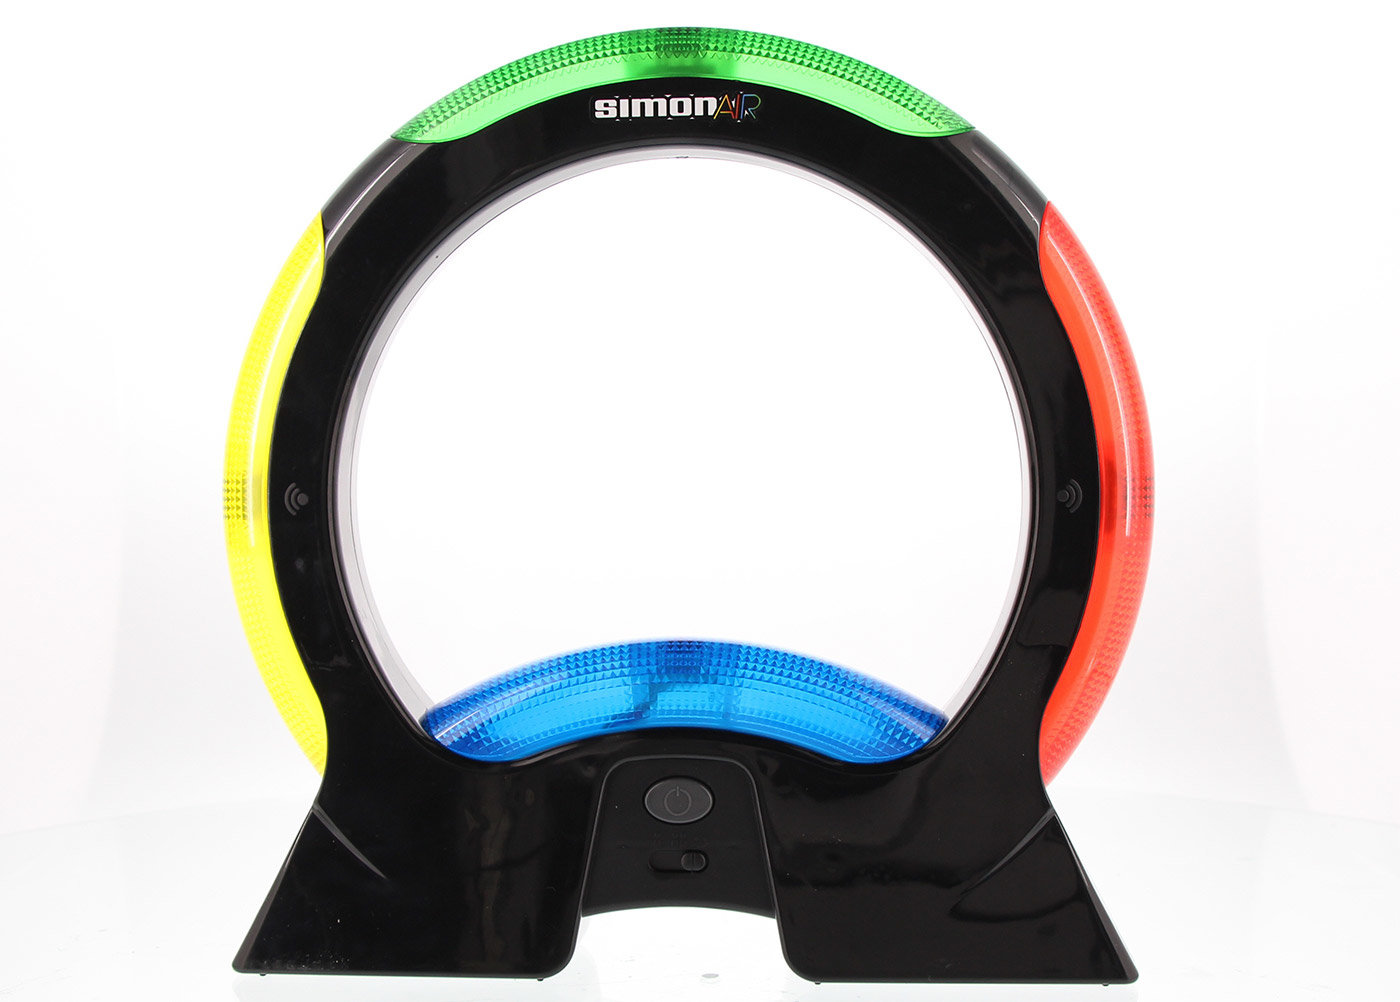
\includegraphics[scale=0.180]{images/simonair_face.jpg}}
        \caption{The Simon game}
        \label{figure1}
    \end{figure}

    The goal for the user is to memorize the order in which the button is lighted, and reproduce it by moving his hand in front of each color (a sensor will detect the hand of the user).
    After succeeding in it, the same sequence will restart, but there will be more buttons's lightning than before.
    The longer the sequence will grow, the harder the game will be.
    If the user fails to reproduce the sequence exactly, the game is over.
    \\

    We developed the same game but in a virtual reality environment (figure \ref{figure2}), in which the concept is the same and the player uses the controller of the VR-system to select a color.
    \begin{figure}[H]
        \centering
        \setlength{\fboxsep}{0pt}
        \fbox{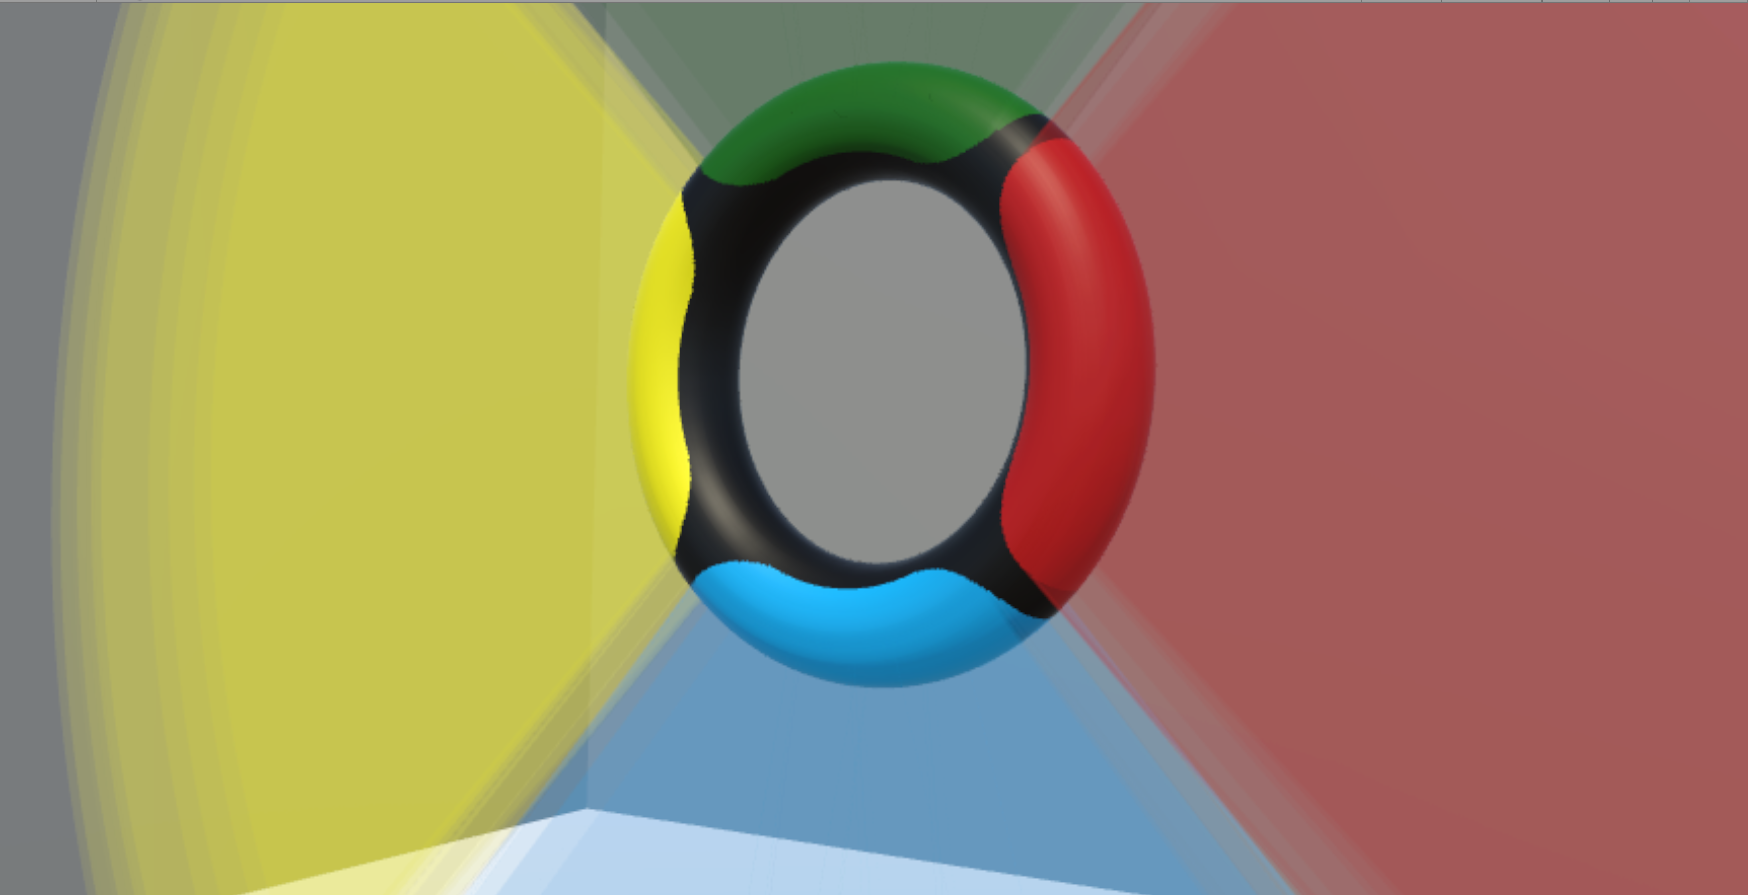
\includegraphics[scale=0.192]{images/simonvr_3d.png}}
        \caption{The VR Simon game}
        \label{figure2}   
    \end{figure}

    \subsection{Test Subjects}
    The experiment is conducted on a sample of 40 people. The age of the subjects varies between fifteen years and thirty years.
    \\

    We don’t make any difference between men and women because we treat symptoms and not a disease that could have different effects regarding the sex of the test subject. All of the test subjects don’t have neither physical nor mental disability.
    
    \subsection{Tools}
        \title{\textbf{The Simon game}} \vspace{0.25cm}

        \noindent The Simon game is a memory board game in which the player has to reproduce the order of lights displayed by the game by, in our version, hovering the colour zone with the hand. \\

        \noindent \title{\textbf{Virtual Reality Headset/Controllers (HTC Vive/Oculus Rift)}} \vspace{0.25cm}

        \noindent With these systems, we are able to create a simulated environment we can control and in which the user can interact. \\
    
        \noindent \title{\textbf{Unity3D}} \vspace{0.25cm}

        \noindent A real-time engine developed by Unity Technologies used to develop (using the C\# language) the 3D environment, allowing user interactions and data analysis. \\

        \noindent \title{\textbf{Blender}} \vspace{0.25cm}

        \noindent A free open-source 3D computer graphics software toolset used to create 3D model. For example here, we reacreated the shape of the Simon board game. \\
        
        \noindent \title{\textbf{Timer}} \vspace{0.25cm}

        \noindent Used by the operator to evaluate the time data of the current player. \\

        \noindent \title{\textbf{Paper/Pen}} \vspace{0.25cm}

        \noindent Used by the operator to write down the observed data of the current player. \\
    
        \noindent \title{\textbf{Statistics Analysis}} \vspace{0.25cm}

        \noindent Used to compile and compare our data.

    \subsection{Protocol}
        \subsubsection{Margin of error}
            \title{\textbf{Goal}} \vspace{0.25cm}

            \noindent Calculate the margin of error of human measurements using stopwatches.
            \\

            \noindent \title{\textbf{Initial conditions}}
                \begin{itemize}
                \renewcommand\labelitemi{--}
                    \item{Requires 4 people, 1 to perform the exercise and 3 to measure its speed of execution.}
                    \item{Needs 3 stopwatches.}
                \end{itemize}

            \noindent \title{\textbf{Protocol}}
                \begin{itemize}
                \renewcommand\labelitemi{--}
                    \item{A person will repeat a serie of 3 colors under the Simon's rules of the game.}
                    \item{Three people measure the reproduction speed of the player's series.}
                    \item{The stopwatches are started when the game displays the first color of the sequence and are stopped when the first color of the next sequence is displayed.}
                    \item{Thanks to an editing software (Adobe Premiere), we measure the time taken by the game to present the sequence to be reproduced and the time taken by the game to restart a sequence of colors after activation of the last color by the player.}
                    \item{These two values are added together and subtracted from the total measured time to obtain the player's time only. Their standard deviations are then calculated to identify the margin of error of the measurements.}
                \end{itemize}
                
        \subsubsection{Virtual Reality}
            \title{\textbf{Goal}} \vspace{0.25cm}

            \noindent Measure the time taken by a user to complete a game and save the related data.
            \\

            \noindent \title{\textbf{Initial conditions}}
                \begin{itemize}
                \renewcommand\labelitemi{--}
                    \item{The test subject has not played the game in the last 48 hours.}
                    \item{A researcher sets up the exercise for the player.}
                \end{itemize}

            \noindent \title{\textbf{Protocol}}
                \begin{itemize}
                \renewcommand\labelitemi{--}
                    \item{The rules of the game are explained to the player: a sequence of colours will appear; the player will have to reproduce this same sequence without error. If it succeeds, the sequence will be one color longer. The player must go as far as possible in the game without making mistakes.}
                    \item{A session is composed of a game done by the player and his results saved in a log file.}
                    \item{The player tests the game once before starting the timed session.}
                    \item{The player does 2 sessions.}
                \end{itemize}

        \subsubsection{Physical}
            \title{\textbf{Goal}} \vspace{0.25cm}

            \noindent Measure the time taken by a user to complete a game and save the related data.
            \\

            \noindent \title{\textbf{Initial conditions}}
                \begin{itemize}
                \renewcommand\labelitemi{--}
                    \item{The test subject has not played the game in the last 48 hours.}
                    \item{We need 2 researchers with one stopwatch each, who will measure the duration of each level.}
                \end{itemize}
            
            \noindent \title{\textbf{Protocol}}
                \begin{itemize}
                \renewcommand\labelitemi{--}
                    \item{The rules of the game are explained to the player : A sequence of colours will appear; the player will have to reproduce this same sequence without error. If it succeeds, the sequence will be one color longer. The player must go as far as possible in the game without making mistakes.}
                    \item{A session is composed of a game done by the player and his results saved into a spreadsheet.}
                    \item{The player tests the game once before starting the timed session.}  
                    \item{The player starts a session.}
                    \item{The researchers start the stopwatch when the first color appears in the example sequence.} 
                    \item{A ``step'' is made each time the first color of the example sequence of a level appears.} 
                    \item{When the player loses, the measured data is saved into a spreadsheet.} 
                    \item{The player does a second session.}
                    \item{The researchers measure the time the same way they did for the first session.}
                \end{itemize}
    % For the first group, we use the physical version of the game.
    % While a person is playing, a second person (the operator) will write down the different parameters we need for the data analysis (see \ref{data}).
    % \\
    
    % For the second group, we use the same version of the board game but in the VR environment.
    % We don't need an operator here, the application will automatically register the needed data.
    % \\

    % Finally, for the third group, we first use the physical version. Then we wait one week before making them play the VR game. Indeed, if they directly try the VR version right after this, it could change their way of playing the game in the VR environment (they would be more efficient).
    % At the end, we compare the data of all of the three groups.

\section{Results}
%All these statistics will be measured by the VR captors and environment.
    
%- Speed : How long does it take  for the user to reproduce the sequence (comparing to the actual duration of the original sequence) ?
%- Efficiency: How long is the sequence remembered by the patient ? Difference between the first session and the Nth session.
%- Accessibility :  How easy it is to install, and play the game ? To record the data ?
   
%We now analyze the data from all of the tests we run during this experiment, displayed in different kinds of graphics \\ %TODO A CHANGER
The box plot graphics, although based on all of the test subjects, only highlight 50\% of them. Those 50\% were chosen because they are close to the median value. 
Indeed, the two colored boxes represent the interquartile range (or middle 50\%), which is a robust statistical dispersion measure, which helps to avoid having too much dispersion when analysing data. Thus, it allows us to get a more representative point of view of the results obtained during our tests. 
\\

    \subsection{Memory performances}
    % - efficiency
    We begin by looking into the memory performances at different times of the experiment.
    Indeed, if the training is successful, we should see an improvement in the amount of colors the test subject is able to memorize before finishing the game.
    \\

        \subsubsection{Short-term memorization}
        First, we analyze the number of colors memorized on the short-term, which means during the first session of the experiment (for both VR and Physical game).
        \\
     
            \noindent \title{\textbf{VR Session}} \vspace{0.25cm}

            % moyenne
            Using VR, the average number of color memorized by the test subjects is 8.75 for the first test and 9.65 for the second test.

            % box plot
                \begin{figure}[H]
                    \centering
                    \setlength{\fboxsep}{0pt}
                    \fbox{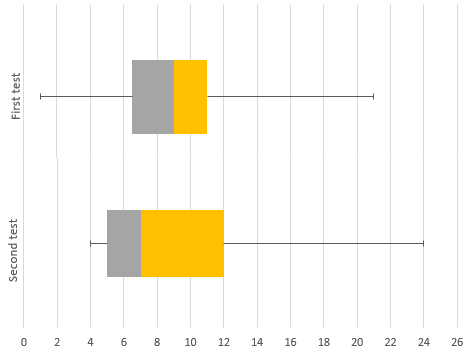
\includegraphics[scale=0.65]{graphics/boxplot-vr-firstandsecondtest.png}}
                    \caption{Box plots of the first and second test of the first VR session}
                    \label{figure3}
                \end{figure}

            This box plot graphic shows us, for each test, the range of levels reached (figure \ref{figure3}).
            We see two boxes on each side of the median value of this range.
            For the first test the subjects complete between 1 and 21 levels during the game. 
            The median has a value of 9, and 25\% of the chosen subjects reach between the 6th and the 9th level while the other 25\% reach between the 9th and the 11th level.
            During the second test, we see that the range of levels completed is from 4 to 24.
            The median value is now 7, and while 25\% of the subjects complete between the 5th and the 7th level, the other 25\% only reach either the 7th or the 12th level.
            \\

            % Nbr de personnes/score
                \begin{figure}[H]
                    \centering
                    \setlength{\fboxsep}{0pt}
                    \fbox{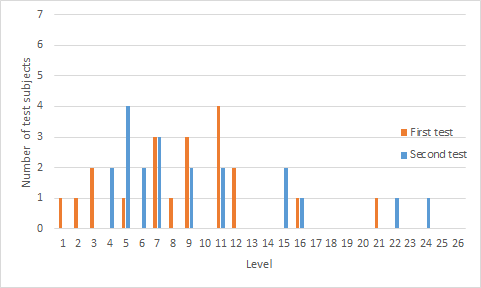
\includegraphics[scale=0.70]{graphics/bargraph-vr-nbtestsubjectperlevel.png}}
                    \caption{Number of test subjects by levels reached for the first VR session}
                    \label{figure4}
                \end{figure}

            In this bar graph (figure \ref{figure4}) we see the results of the first and second test, for the first session in VR.
            For the first test, nobody completes more than 21 levels, with a minimum of levels reached of 1.
            We can see three different groups in these results.
            25\% of the test subjects complete the levels between 1 and 5.
            The majority of the test subjects (65\%) reaches between the 7th and the 12th level.
            Only two test subjects (10\%) complete the 16th and the 21st level.
            For the second test, only two test subjects (10\%) complete more than 21 levels, three of the group (15\%) complete between 15 and 16 levels. 
            But for 75\% of the group, the levels reached are between 4 and 11.
            
            % Progression
                \begin{figure}[H]
                    \centering
                    \setlength{\fboxsep}{0pt}
                    \fbox{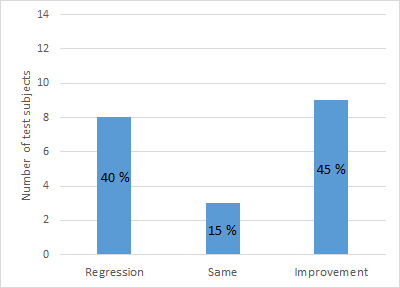
\includegraphics[scale=0.86]{graphics/rsi-vr.png}}
                    \caption{Progression of the test subjects between the two tests for the first VR session}
                    \label{figure5}
                \end{figure}

            In this bar graph (figure \ref{figure5}) we see that, for the two tests of the first VR session, 40\% of the subjects made, during the second test, a worse score than the first one. 
            15\% made the same score and 45\% made a better score.
            \\

            \noindent \title{\textbf{Physical Session}} \vspace{0.25cm}

            % moyenne
            Using the physical game, the average number of colors memorized by the test subjects is 7.85 for the first test and 6.5 for the second test.
          
            % box plot
                \begin{figure}[H]
                    \centering
                    \setlength{\fboxsep}{0pt}
                    \fbox{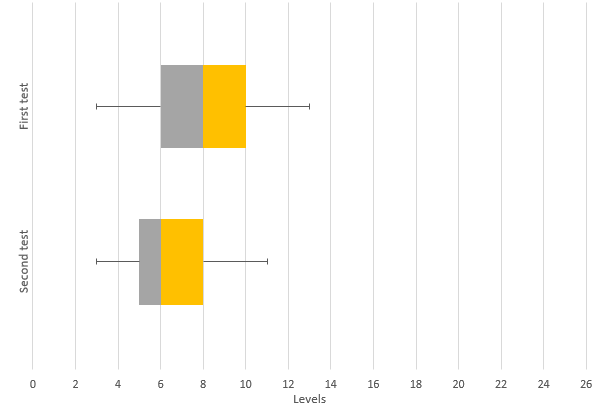
\includegraphics[scale=0.74]{graphics/boxplot-p-firstandsecondtest.png}}
                    \caption{Box plots of the first and second test of the first physical session}
                    \label{figure6}
                \end{figure}
        
            This box plot graphic shows us, for each test, the range of levels reached (figure \ref{figure6}).
            We see two boxes on each side of the median value of this range.
            For the first test the subjects complete between 3 and 13 levels during the game. 
            The median has a value of 8, and 25\% of the chosen subjects reach between the 6th and the 8th level while the other 25\% reach between the 8th and the 10th level. 
            During the second test, we see that the range of levels completed is from 3 to 11. 
            The median value is now 6, and while 25\% of the subjects complete between the 6th and the 8th level, the other 25\% only reach either the 5th or the 6th level.
            \\

            % Nbr de personnes/score
                \begin{figure}[H]
                    \centering
                    \setlength{\fboxsep}{0pt}
                    \fbox{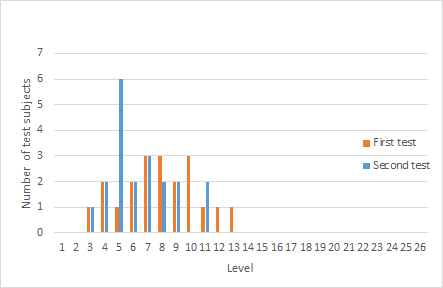
\includegraphics[scale=0.74]{graphics/bargraph-p-nbtestsubjectperlevel.png}}
                    \caption{Number of test subjects by levels reached for the first physical session}
                    \label{figure7}
                \end{figure}
            In this bar graph (figure \ref{figure7}) we see the results of the first and second test, for the first session with the physical version of the game.
            For the first test, nobody completes more than 13 levels, with a minimum of levels reached of 3.
            The test subjects are almost equally distributed in this range of levels.  
            We still observe peaks at the 7th, the 8th and the 10th levels (45\% of the test subjects reach these levels).
            For the second test, nobody completes more than 11 levels, with a minimum of levels reached of 3. 
            We observe a peak at the fifth level reached by 6 test subjects, which is 30\% of the whole group.
            \\
        
            % Progression
                \begin{figure}[H]
                    \centering
                    \setlength{\fboxsep}{0pt}
                    \fbox{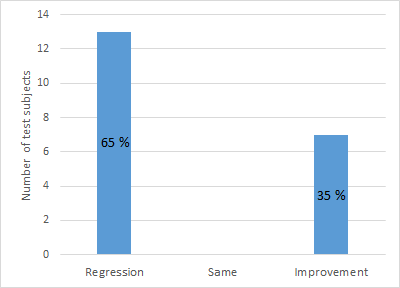
\includegraphics[scale=0.84]{graphics/rsi-p.png}}
                    \caption{Progression of the test subjects between the two tests for the first physical session}
                    \label{figure8}
                \end{figure}

            In this bar graph (figure \ref{figure8}) we see that, for the two tests of the first physical session, only 35\% of the test subjects improve their score. 
            The 65\% left have all made a worse score than during their first test.
       
        \subsubsection{Long-term memorization}
        Then, we look into the same data but on the long term (both sessions) by group.
        \\
    
            \noindent \title{\textbf{VR-VR Group}}
            % box plot
                \begin{figure}[H]
                    \centering
                    \setlength{\fboxsep}{0pt}
                    \fbox{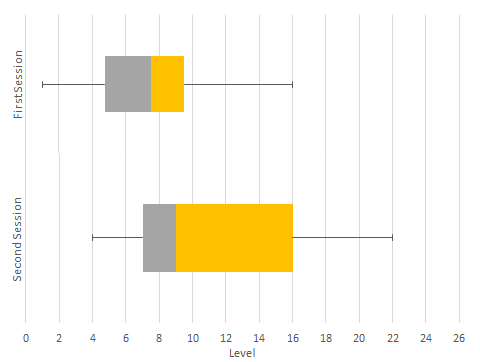
\includegraphics[scale=0.64]{graphics/boxplot-vrvr-12session.png}}
                    \caption{Box plots of the first and second session for VR}
                    \label{figure9}
                \end{figure}

            This box plot graphic shows us, for each one of the two sessions (two tests by session), the range of levels reached (figure \ref{figure9}).
            We see two boxes on each side of the median value of this range.
            For the first session the subjects complete between 1 and 16 levels.
            The median has a value of 7.5, and 25\% of the chosen subjects reach between the 5th and the 7th/8th level, while the other 25\% reach between the 7th/8th level and the 9th/10th level.
            During the second session, we see that the range of levels completed is from 4 to 22. The median value is now 9, and while 25\% of the subjects only complete between the 5th and the 9th level, the other 25\% reach from 9 to 16 levels.
            
            % Progression
                \begin{figure}[H]
                    \centering
                    \setlength{\fboxsep}{0pt}
                    \fbox{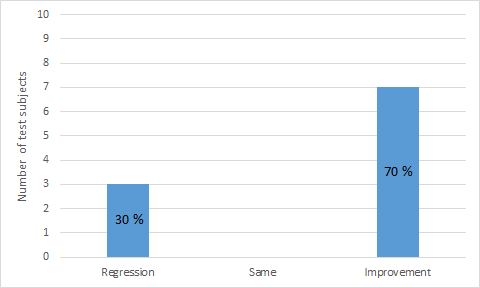
\includegraphics[scale=0.64]{graphics/rsi-vrvr.png}}
                    \caption{Progression of the test subjects between the first and the second session for VR}
                    \label{figure10}
                \end{figure}

            In this bar graph (figure \ref{figure10}) we see that, for the two VR sessions, only 30\% of the test subjects have a worse score during their second session. 
            70\% of them have a better score.
            \\

            \noindent \title{\textbf{Physical-Physical Group}}           
            % box plot
                \begin{figure}[H]
                    \centering
                    \setlength{\fboxsep}{0pt}
                    \fbox{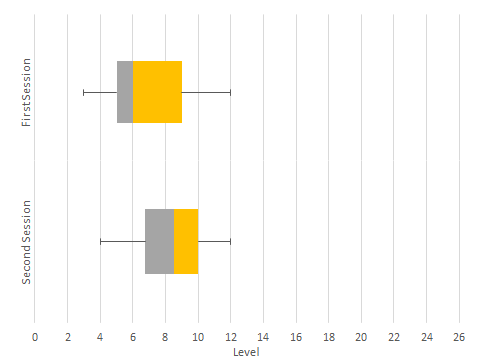
\includegraphics[scale=0.58]{graphics/boxplot-pp-12session.png}}
                    \caption{Box plots of the first and second session for the physical game}
                    \label{figure11}
                \end{figure}

            This box plot graphic (figure \ref{figure11}) shows us, for each one of the physical session, the range of levels reached. We see two boxes on each side of the median value of this range.
            For the first session, the subjects complete between 3 and 12 levels. The median has a value of 6, and 25\% of the chosen subjects only reach the 5th/6th level. The other 25\% complete between the 6th and 9th level.
            For the second session, we see that the range of levels completed is from 4 to 12. The median value is now 8.5, and while 25\% of the subjects complete between the 7th and the 8th/9th level, the other 25\% reach from the 8th/9th and the 10th level.
                
            % Progression
                \begin{figure}[H]
                    \centering
                    \setlength{\fboxsep}{0pt}
                    \fbox{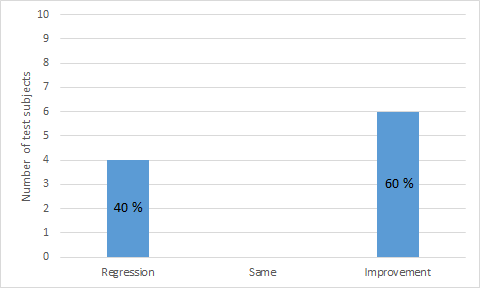
\includegraphics[scale=0.58]{graphics/rsi-pp.png}}
                    \caption{Progression of the test subjects between the first and the second session for the physical game}
                    \label{figure12}
                \end{figure}

            In this bar graph (figure \ref{figure12}) we see that, for the two physical sessions, 40\% of the test subjects have a worse score during their second session.
            60\% of them have a better score.
            \\

            \noindent \title{\textbf{VR-Physical Group}}
            % box plot
                \begin{figure}[H]
                    \centering
                    \setlength{\fboxsep}{0pt}
                    \fbox{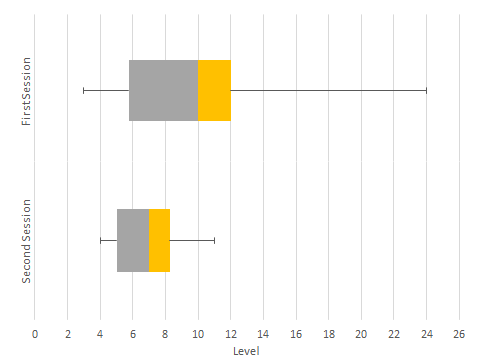
\includegraphics[scale=0.58]{graphics/boxplot-vrp-12session.png}}
                    \caption{Box plots of the first session (on the VR game) and the second session (on the physical game)}
                    \label{figure13}
                \end{figure}

            This box plot graphic (figure \ref{figure13}) shows us, for each session (A first session in VR, the next one with the physical game), the range of levels reached. We see two boxes on each side of the median value of this range.
            For the first session, in VR, the subjects complete between 3 and 24 levels. The median has a value of 10, and 25\% of the chosen subjects reach between the 5th/6th and the 10th level. The other 25\% complete between the 10th and the 12th level.
            For the second session, with the physical version of the game, we see that the range of levels completed is from 4 to 11. The median value is now 7, and while 25\% of the subjects complete between the 5th and the 7th level, the other 25\% reach from the 7th to the 8th/9th level.

            % Progression
                \begin{figure}[H]
                    \centering
                    \setlength{\fboxsep}{0pt}
                    \fbox{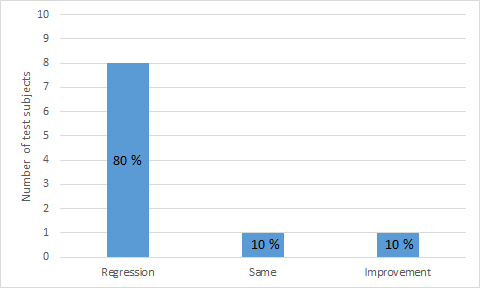
\includegraphics[scale=0.62]{graphics/rsi-vrp.png}}
                    \caption{Progression of the test subjects between the first session (on the VR game) and the second session (on the physical game)}
                    \label{figure14}
                \end{figure}

            In this bar graph (figure \ref{figure14}) we see that, for the two sessions (first session in VR, then with the physical version), a majority of 80\% of test subjects see a regression in their score, while 10\% remain with the same score, and another 10\% have a better score.
            \\

            \noindent \title{\textbf{Physical-VR Group}}          
            % box plot
                \begin{figure}[H]
                    \centering
                    \setlength{\fboxsep}{0pt}
                    \fbox{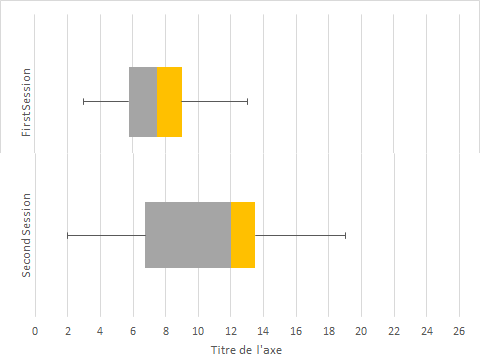
\includegraphics[scale=0.68]{graphics/boxplot-pvr-12session.png}}
                    \caption{Box plots of the first session (on the physical game) and the second session (on the VR game)}
                    \label{figure15}
                \end{figure}
            
            This box plot graphic shows us, for each session (A first session with the physical game, the next one in VR), the range of levels reached (figure \ref{figure15}).
            We see two boxes on each side of the median value of this range.
            For the first session, with the physical version of the game, the subjects complete between 3 and 13 levels. The median has a value of 7.5, and 25\% of the chosen subjects reach between the 5th/6th and the 7th/8th level. The other 25\% complete between the 7th/8th and the 9th level.
            For the second session, in VR, we see that the range of levels completed is from 2 to 19. The median value is now 12, and while 25\% of the subjects complete between the 5th and the 12th level, the other 25\% reach from the 12th to the 13th/14th level.

            % Progression
                \begin{figure}[H]
                    \centering
                    \setlength{\fboxsep}{0pt}
                    \fbox{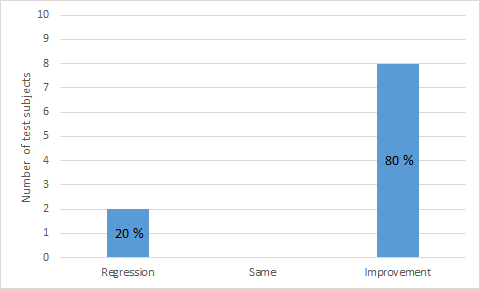
\includegraphics[scale=0.65]{graphics/rsi-pvr.png}}
                    \caption{Progression of the test subjects between the first session (on the physical game) and the second session (on the VR game)}
                    \label{figure16}
                \end{figure}

            In this bar graph (figure \ref{figure16}) we see that, for the two sessions (first session with the physical version, then in VR), a majority of 80\% of test subjects see an improvement in their score, while 20\% have a better score.
            \\

            \noindent \title{\textbf{Comparison between VR and physical results}} \vspace{0.25cm}

            \noindent Finally, we compare the data for the two different technologies used in order to see which is the best technology for learning. \\

            % box plot
                \begin{figure}[H]
                    \centering
                    \setlength{\fboxsep}{0pt}
                    \fbox{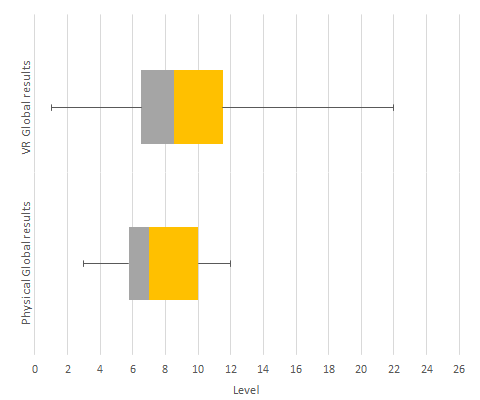
\includegraphics[scale=0.65]{graphics/boxplot-vr-p-globalresults.png}}
                    \caption{Box plots of all the sessions combined per technology}
                    \label{figure17}
                \end{figure}

            This box plot graphic (figure \ref{figure17}) shows us, for each one of the technologies used (including every tests/sessions for the VR/VR and the Physical/Physical groups), the range of levels reached. We see two boxes on each side of the median value of this range.
            For the VR sessions, the subjects complete between 1 and 22 levels. The median has a value of 8.5, and 25\% of the chosen subjects reach between the 6th/7th and the 8th/9th level, while the other 25\% reach between the 8th/9th and the 11th/12th level.
            For the physical sessions, we see that the range of levels completed is from 3 to 12. The median value is now 7, and while 25\% of the subjects only complete between the 5th and the 7th level, the other 25\% reach from 7 to 10 levels.

            % box plot
                \begin{figure}[H]
                    \centering
                    \setlength{\fboxsep}{0pt}
                    \fbox{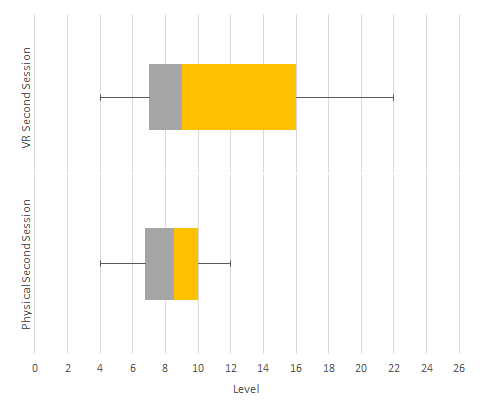
\includegraphics[scale=0.65]{graphics/boxplot-vr-p-session2results.png}}
                    \caption{Box plots of the session two per technology}
                    \label{figure18}
                \end{figure}

            This box plot graphic shows us, for each one of the technologies used, the range of levels reached for each technology's second session (figure \ref{figure18}). We see two boxes on each side of the median value of this range.
            For the VR second session, the subjects complete between 4 and 22 levels. The median has a value of 9, and 25\% of the chosen subjects reach between the 7th and the 9th level. The other 25\% reach between the 9th and the 16th level.
            For the second physical session, we see that the range of levels completed is from 4 to 12. The median value is now 8.5, and while 25\% of the subjects complete between the 7th and the 8th/9th level, the other 25\% reach from the 8th/9th and the 10th level.

    \subsection{Speed of execution}
    %- Speed
    The second part of this analysis is about the speed of execution.
    If the training is successful, we should see an improvement in the test subject's speed of execution of the different exercises. We decided to study the execution speed for the level three and six in order to display relevant results. The level three has been chosen because most people reach it and the level six because it is a level a bit more difficult to reach (but which still allows to analyse data). 
        \subsubsection{Short-term speed execution}
        First, we analyze the speed of execution on the short-term, which means during the first session of the experiment (for both VR and Physical game).
        \\

            \noindent \title{\textbf{First VR Session}} \vspace{0.25cm}
            
            % Progression
            Using the VR game, the average speed of execution is 3.437 seconds for the level three and 6.606 seconds for the level six.

            % Speed 3
                \begin{figure}[H]
                    \centering
                    \setlength{\fboxsep}{0pt}
                    \fbox{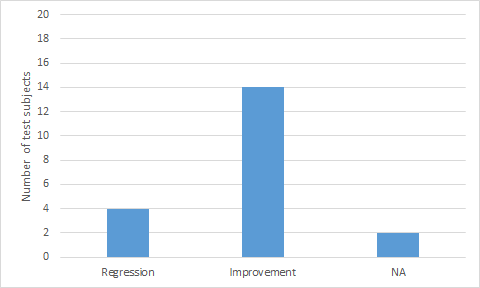
\includegraphics[scale=0.70]{graphics/rsi-vr-speed3.png}}
                    \caption{Progression of the execution speed of the test subjects for the first VR session (Level 3)}
                    \label{figure19}
                \end{figure}

            In this bar graph (figure \ref{figure19}), we evaluate the difference in execution speed between the two tests of the first VR session, for the third level. 
            We see that great majority of the test subjects (70\%) improve their execution speed while 20\% of them reduce it, and 10\% don't reach this level.
            \\

            % Speed 6
                \begin{figure}[H]
                    \centering
                    \setlength{\fboxsep}{0pt}
                    \fbox{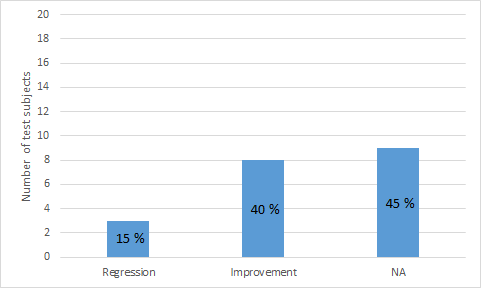
\includegraphics[scale=0.70]{graphics/rsi-vr-speed6.png}}
                    \caption{Progression of the execution speed of the test subjects for the first VR session (Level 6)}
                    \label{figure20}
                \end{figure}
        
            In this bar graph (figure \ref{figure20}), we evaluate the difference in execution speed between the two tests of the first VR session, for the sixth level. 
            While 45\% of the test subjects don't reach the 6th level, 40\% of them see an improvement in their execution speed. Only 15\% observe a regression for it.
            \\

            \noindent \title{\textbf{First Physical Session}}  \vspace{0.25cm}
            
            % Progression
            Using the physical game, the average speed of execution is 2.501 seconds for the level three and 4.113 seconds for the level six.

            % Speed 3
                \begin{figure}[H]
                    \centering
                    \setlength{\fboxsep}{0pt}
                    \fbox{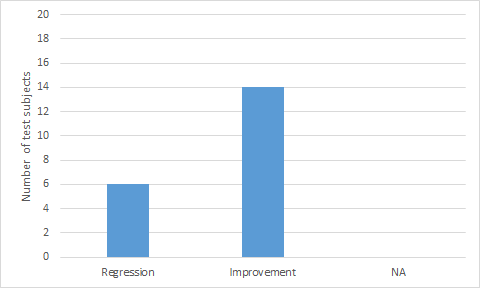
\includegraphics[scale=0.70]{graphics/rsi-p-speed3.png}}
                    \caption{Progression of the execution speed of the test subjects for the first physical session (Level 3)}
                    \label{figure21}
                \end{figure}

            In this bar graph (figure \ref{figure21}), we evaluate the difference in execution speed between the two tests of the first physical session, for the third level.
            We observe that 70\% of the test subjects reduce their execution speed during the second test, while 30\% of them have a longer execution speed.

            % Speed 6
                \begin{figure}[H]
                    \centering
                    \setlength{\fboxsep}{0pt}
                    \fbox{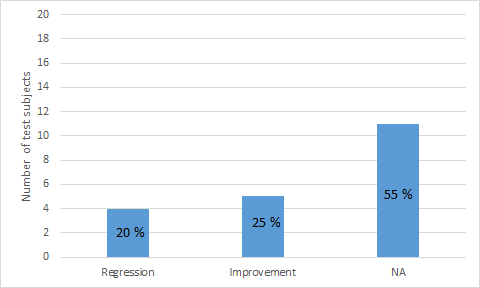
\includegraphics[scale=0.70]{graphics/rsi-p-speed6.png}}
                    \caption{Progression of the execution speed of the test subjects for the first physical session (Level 6)}
                    \label{figure22}
                \end{figure}

            In this bar graph (figure \ref{figure22}), we evaluate the difference in execution speed between the two tests of the first physical session, for the sixth level.
            We see that only 25\% of the test subjects reduce their execution speed, and 20\% have a longer one. Most of the test subjects (55\%) don't reach the 6th level.

    \subsubsection{Long-term speed execution}

    \noindent \title{\textbf{Physical-Physical Group}} \vspace{0.25cm}

    Using the physical game, for the first session, the average speed of execution is 2.423 seconds for the level three and 3.544 seconds for the level six. For the second session, the average speed of execution is  2,055 seconds for the level three and 3.957 seconds for the level six.
    \\

    \noindent \title{\textbf{VR-VR Group}} \vspace{0.25cm}
    
    For the first session of the VR game, the average speed of execution is 3.673 seconds for the level three and 7.449 seconds for the level six. However, for the second session, the average speed of execution is 2.917 seconds for the level three and 5.962 seconds for the level six.
    \\
    
    \noindent \title{\textbf{VR-Physical Group}} \vspace{0.25cm}
    
    For the first session (the VR game), the average speed of execution is 3.220 seconds for the level three and 7.199 seconds for the level six. Whereas, for the second session (the physical game), the average speed of execution is 2.134 seconds for the level three and 4.461 seconds for the level six.
    \\

    \noindent \title{\textbf{Physical-VR Group}} \vspace{0.25cm}
    
    For the first session (the physical game), the average speed of execution is 2.178 seconds for the level three and 3.992 seconds for the level six. Whereas, for the second session (the VR game), the average speed of execution is 3.140 seconds for the level three and 6.573 seconds for the level six.
    \\
 

    %accessibility
    %The training, supposed to be done at home by anyone, should be easy, from the setup of the environment to the actual beggining of the game. 
    %We can measure here the time spent on the different interface pannels and how much time the user spends to setup the machine, with the help of our instructions.

\section{Conclusion}
    In this conclusion, we present what can be deduced from the different data available following the two training sessions.
    \\

    First of all, the data provided by the test subjects help us to learn more about the differences in terms of memory performance.
    \\

    On the short term (for the first session), there is a difference between the test subjects in Virtual Reality and with the physical version of the game.
    We see an improvement of the memory performances during the first VR session rather than in the first physical session. Indeed, in VR, the range of levels reached is incremented by 3 (for the minimum and the maximum levels completed), whereas in the physical version we don't see any changes, the maximum level reached is even lower (2 levels less) during the second test. 
    In this same session, for the chosen 50\% of test subjects we study, the test subjects did a better score in the first test than at the second one. The median decreased from 8 to 6, which represent a loss of score, in general.
    However, in the VR session, the chosen 50\%, although having more variable results during the second test, see some of their scores increased, despite a majority of scores being worse than in the first test: the median decreased from 9 to 7 at the second test. 
    But we better see the difference between the two technologies while looking at the progression percentage between the scores of the two tests. In the physical session we have 65\% of regression for only 35\% of improvement, as the average score of players decreased from 7.85 to 6.5 between first and second test of the first session.
    On the contrary, in VR, we may see 40\% of regression, but we also see 45\% of improvement, as the average score of players increased from 8.75 to 9.65 between first and second test of the first session.
    So we notice a slight advantage in VR compared to the physical version on the short term. Indeed we notice an improvement of the memory performances.
    This difference can be explained, despite the different technologies used, by the boredom and difficulty to concentrate after playing for more than a few minutes to the physical version, which may happen less times in Virtual Reality as we are completely immersed in the environment, althought it is possible, as some test subjects claim, that the use of a screen can be tiring for their eyes. 
    \\
    
    On the long term, the differences are even bigger. 
    For the group which did both sessions in VR. The results show a really good improvement. Between the first and second session, the range of levels reached is incremented
    by 3 for the minimum level reached, and 6 for the maximum level reached. 
    The chosen 50\% of tests subjects we study, in addition of having more variable results in the second session, some of them have the same score but most of them have a better one. 
    Obviously, this improvement can also be seen in the percentages of the total progression. For only 30\% of regression, we notice a 70\% improvement in the test subjects' results between the two session.
    We see here, while doing both session in VR, a great improvement.  
    \\
    For another group (VR/Physical), which did the first session in VR and the second session with the physical version of the game, there is also a great change between the two session.
    The range of levels reached change between the first session in VR and the second session with the physical version, although the minimum level reached is incremented by 1, the maximum level reached is greatly lowered by 13.
    The chosen 50\% test subjects have closer scores in the second session, but none of them has a better score. If we look into the total progression percentages, we see a little 10\% of improvement for 80\% of regression.
    What we notice here is that, despite having quiet good results during the first session in VR, a great majority of the test subjects had a difficult time during the second session with the physical version. During the tests, they often claimed it was better and easier for them to play this game in virtual reality.
    \\
    For the Physical/Physical group, which did both sessions with the physical version of the game, the range of level reached don't change a lot between the two session. The minimum level reached is incremented by 1 but the maximum level reached doesn't change. 
    For the chosen 50\% test subjects, they have closer scores during the second session, and overall they have a better score. For the total progression percentages, 40\% of the test subjects have a lower score and 60\% have a better one during the second test. 
    We notice that, despite having an overall improvement in their results, this group still doesn't reach an higher percentage of improvement than the group which did both sessions in VR. 
    \\
    For the Physical/VR group, the minimum level reached decreased from the level 3 to the level 2 but the median value increased, it gained 5 level (changed from 7 to 12). The maximum level reached is also way higher in Virtual Reality (6 levels more in VR). 
    In fact, using the VR game leads to an improvement for most part of the test subjects during the second session. Indeed, we notice that 80\% of them improved while only 20\% of them did a lower score during the second session.
    \\

    Regarding the technologies, with the results of all the groups in all the session, we globally see better results in virtual reality. Indeed, we have the lowest score of all the groups (only one level reached by someone), but it is someone who didn't really understood how the game works in VR during the first test. On the other hand the maximum level reached is way higher in VR (10 levels higher), which means that people were a bit more capable of running a very high score in VR than in the physical game.
    Overall, the chosen 50\%, have a difference of one level between the VR results and the physical results. Regarding the median, it is 1.5 higher in VR. Which shows a slightly better memory performance in VR. 
    The results for the second sessions between the VR/VR group and the Physical/Physical group show us that the VR group has better results. Indeed, the minimum level reached is the same for both technology but the chosen 50\% in VR have more variable scores, and a maximum score 4 level higher than the chosen 50\% with the physical version of the game, which means people are better using VR. 
    \\
    
    The execution speed of the physical and virtual exercise are different. For the physical measures, we included an error margin of 0.067 seconds calculated using the standard deviation. This standard deviation was made on a training session (different from the actual test sessions).
    For both the VR and physical exercise, at level 3, 70\% of players improved their speed of execution between first and second test of the session. Whereas for level 6, 40\% of VR players increased their speed, while 25\% of physical players increased their speed.
    For the VR-Physical group, the players increased their time by an average of 1.086 seconds for the third level and 2.738 seconds for the sixth level.
    For the Physical-VR group, the players decreased their time by 0.962 seconds for third level and by 2.581 secondes for sixth level.
    With these results, it seems that physical exercise is generally faster than the virtual one, but there are too many biais to conclude this statement, like the pressure applied by researcher clocking the player, the virtual object looking way bigger than the physical object and the different validation methods.
    \\

    Overall, the VR technology allows for an improvement of the memory performances as explained by previous studies and by the results of our experiment.
    This is mostly due to the VR environment which allows for a more immersive environment. Thanks to this immersive environnement, the test subjects are more receptive and better test conditions (better visibility and concentration).
    Regarding the speed execution, we did not noticed any improvement using VR on both short term and long term. We should do this experiment on a greater period of time.
    We noticed that because of the game and the immersive environment, most people took their time to complete each level instead of doing it as fast as possible.
    \\

    To conclude, we want to add that some parameters may biase our study. Indeed, the total number of participants to this study (40), is a bit small to be really meaningful. 
    Their diversity is not really motley, there are mostly male participants, of a young population, most of them is around twenty years of age. 

\section{Thanks}

The research team would like to thank everyone who made this study possible. We would like to thank Lucie Martinet, our referent, as well as all the test subjects and Cesi for providing us the resources required to carry out this project.

\bibliographystyle{plain}
\bibliography{database}
\end{document}
